\documentclass{beamer}
\title{Snails}
\author{Craig \and Milan \and Jack}
\date{20th June}
\usetheme{AnnArbor}
\usecolortheme{dolphin}
\setbeamertemplate{navigation symbols}{} 

\AtBeginSection
{
  \begin{frame}{Outline}
    \tableofcontents[currentsection]
  \end{frame}
}

\begin{document}

\begin{frame}
  \titlepage
  \vspace{\baselineskip}
  \begin{figure}
    
\includegraphics[scale=0.15]{snail_teeth.png}
  \end{figure}
\end{frame}

\section{Introduction}

\begin{frame}{Introduction}
  We did a game about snails and we think it is pretty cool and you guys should probably check it out or something. \\
  \vspace{\baselineskip}
  I mean, no pressure, but it is pretty awesome.
\end{frame}


\section{The Game}
\subsection{Game Background}

\begin{frame}{Background Story}
  Players are ghosts, in a haunted house which is under attack from evil giant snails.\\
  Ghosts must wear their magic hats at all times to 'live'. The hats magically allow them to interact with the physical world (hold guns, ammo, etc), which also means that the ghosts cannot pass through walls. The hats also magically tie the ghosts to the house - they must haunt the same place forever.\\
  The snails are slightly magical, and are the only things that can kill the ghosts.\\
  \vspace{\baselineskip}
  \begin{figure}
    \hfill
    
\includegraphics[scale=0.15]{snail_teeth_flip.png}
  \end{figure}
\end{frame}

\begin{frame}{Game Rules}
  \begin{itemize}
    \item Ghosts may chose one action to do per turn:
      \begin{itemize}
        \item Move
        \item Shoot
        \item Reload
        \item Pick up or drop the ammo box
        \item Create or fix a barricade
        \item Destroy a barricade
      \end{itemize}
    \item Players have limited ammo, and may not shoot when they have none left
    \item Players carrying the ammo box may only either move or drop the ammo box on their turn
    \item Players may not reload from a carried ammo box
    \item Players may not create or repair a barricade when there are snails in the adjacent room
    \item After each player has had their turn, snails will either chose to chase the nearest player, or move randomly
    \item Ghosts will die when in a room with any number of snails
  \end{itemize}
\end{frame}

\subsection{Aesthetics}

\begin{frame}{Art and Animation}
  \begin{figure}
    \centering
    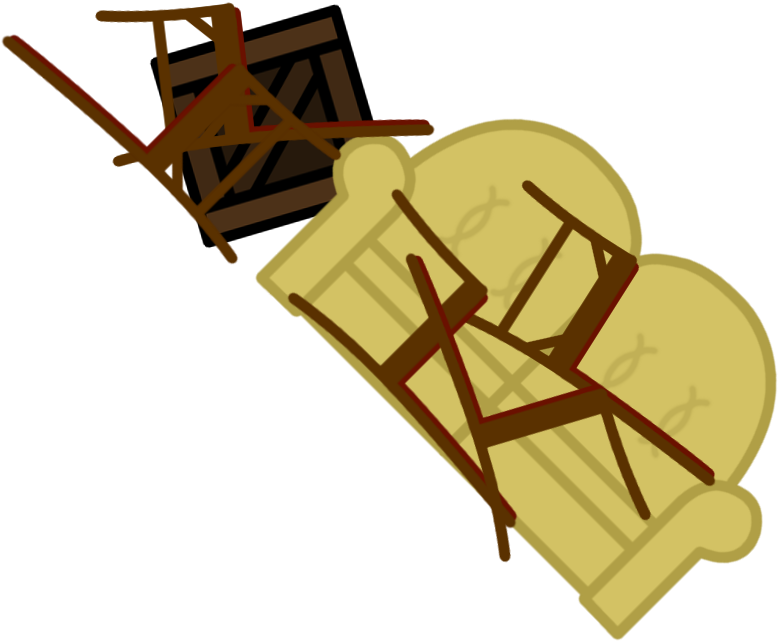
\includegraphics[scale=0.1]{../game/static/img/barricade_stairs.png}
    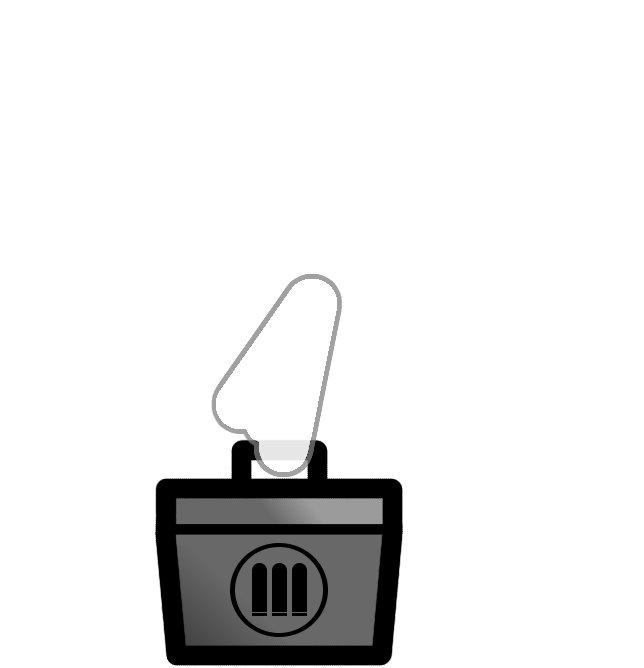
\includegraphics[scale=0.1]{../game/static/img/ghost_ammobox.png}
    
\includegraphics[scale=0.15]{../game/static/img/snail_teeth.png}
    \caption{Various graphics created for the game}
  \end{figure}
  \begin{itemize}
    \item Art - GIMP
    \item Animation - JavaScript/paper.js
  \end{itemize}
\end{frame}

\begin{frame}{User Interface}
  \begin{figure}[hb]
    \centering
    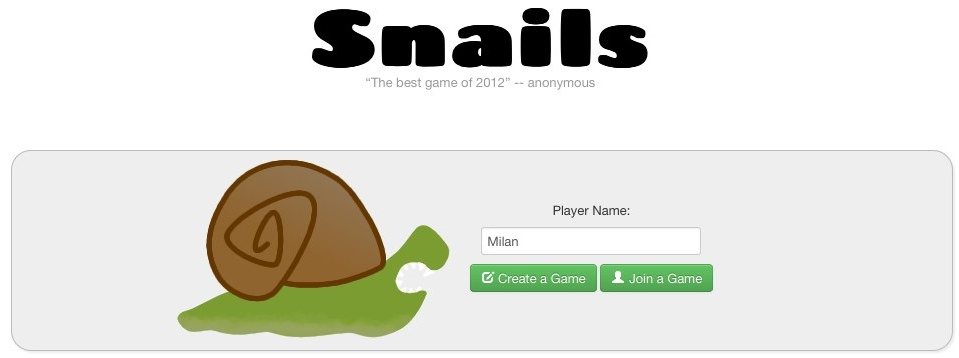
\includegraphics[scale=0.3]{index.jpg}
    \caption{Main screen}
  \end{figure}
\end{frame}

\begin{frame}{User Interface}
  \begin{figure}[hb]
    \centering
    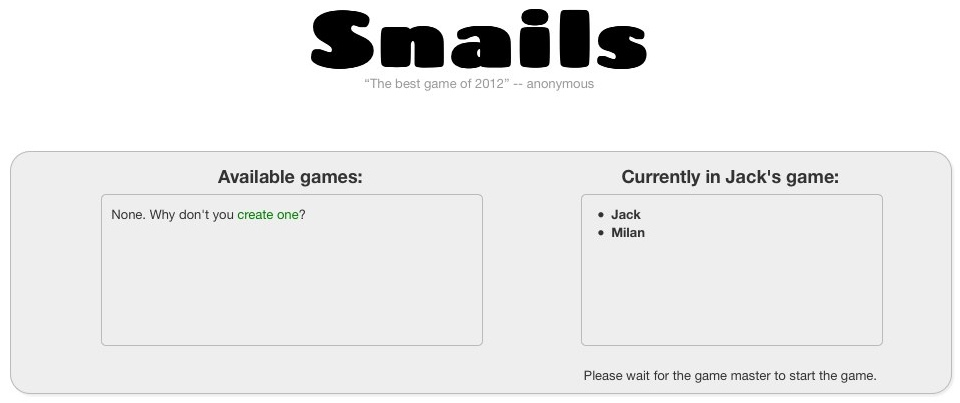
\includegraphics[scale=0.3]{join.jpg}
    \caption{Joining a game}
  \end{figure}
\end{frame}

\begin{frame}{User Interface}
  \begin{figure}[hb]
    \centering
    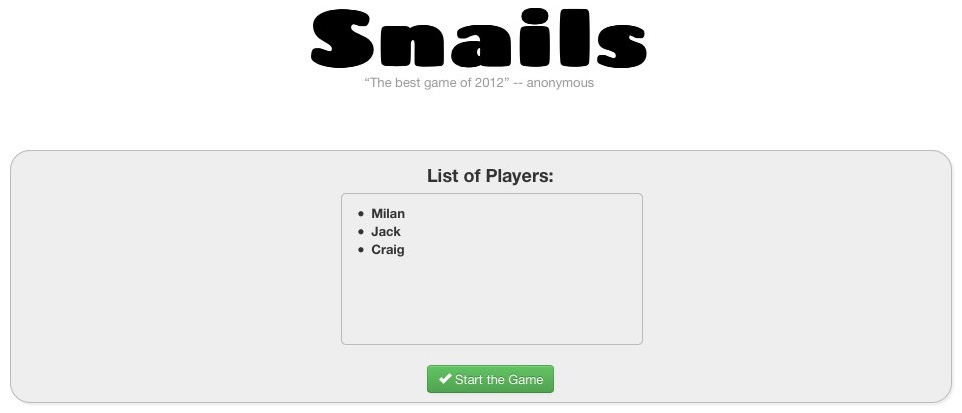
\includegraphics[scale=0.3]{create.jpg}
    \caption{Creating a new game}
  \end{figure}
\end{frame}


\section{Group Management}

\begin{frame}{Git}
\end{frame}

\begin{frame}{Pivotal Tracker}
  Clear structure.\\
  \begin{figure}[hb]
    \centering
    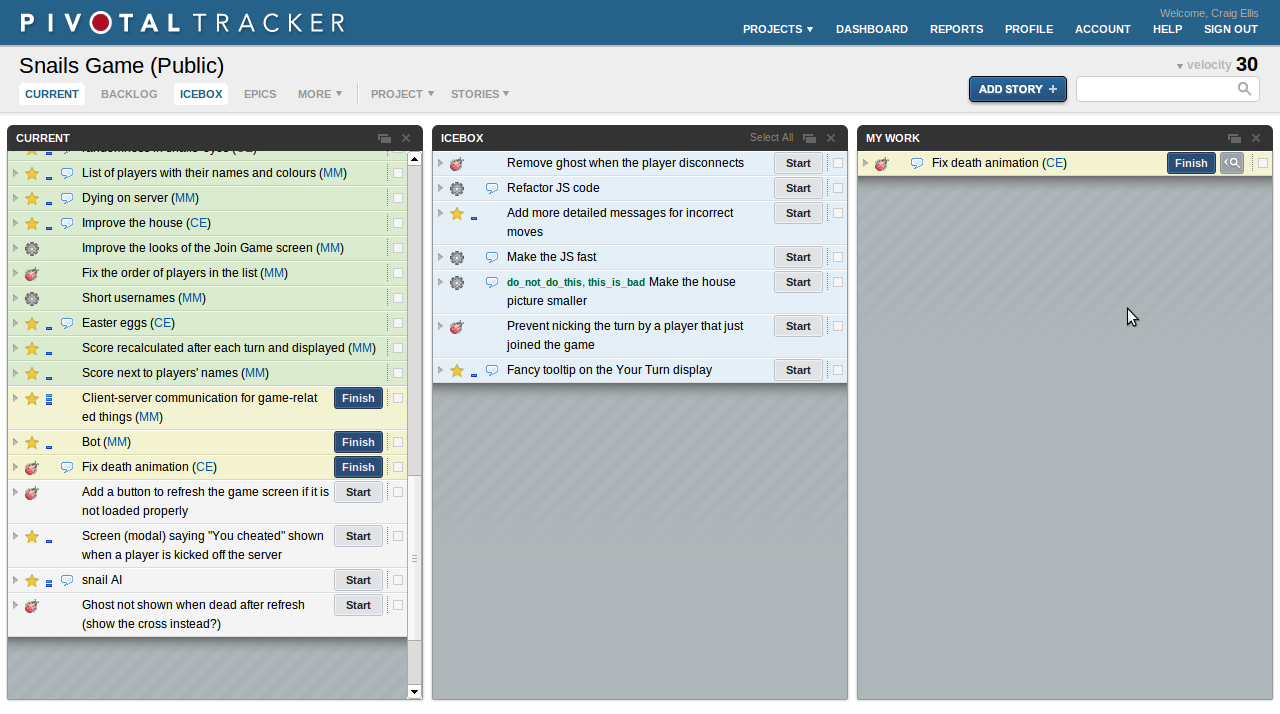
\includegraphics[scale=0.2]{pivotal.png}
    \caption{Pivotal Tracker main screen}
  \end{figure}
\end{frame}

\begin{frame}{Pivotal Tracker}
  Clear structure.\\
  \begin{figure}[hb]
    \centering
    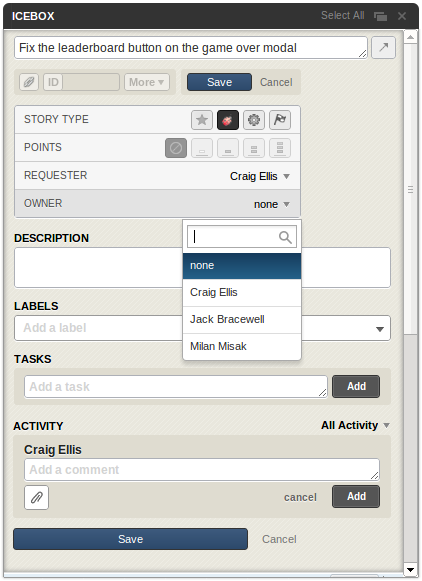
\includegraphics[scale=0.25]{pivotal_new_story.png}
    \caption{Creating a new story}
  \end{figure}
\end{frame}


\section{Implementation Languages}
\subsection{Client}

\begin{frame}{Javascript}
  [insert map of components and interactions.]
  \begin{itemize}
    \item Only client side script supported by all browsers
    \item More stable than using plugins
    \item HTML5 graphics libraries available (we used paper.js)
  \end{itemize}
\end{frame}

\begin{frame}{HTML5}
  [insert map of components and interactions.]
  \begin{itemize}
    \item Technology for the future.
    \item No need to install plugins with modern broswers.
    \item Faster, less likely to crash than plugins.
  \end{itemize}
\end{frame}

\subsection{Server}

\begin{frame}{Django}
  [insert map of components and interactions.]
  \begin{itemize}
    \item Easy ajax.
    \item It's nice
    \item We like it
  \end{itemize}
\end{frame}

\begin{frame}{Heroku}
  [insert map of components and interactions.]
  \begin{itemize}
    \item Free hosting service available.
    \item Supports Django, unlike doc.
    \item Easy deployment - just push to a git repository.
  \end{itemize}
\end{frame}


\section{Conclusion}

\begin{frame}{Conclusion}
  [insert reflection on project outcomes.]
\end{frame}

\end{document}
